\documentclass[conference,a4paper]{IEEEtran}
\IEEEoverridecommandlockouts
\usepackage{cite}
\usepackage{amsmath,amssymb}
\usepackage{graphicx}
\graphicspath{{./}{../figures/}}
\usepackage{booktabs}
\usepackage{array}
\usepackage{tabularx}
\usepackage{xcolor}
\usepackage{tikz}
\usetikzlibrary{positioning,arrows.meta,calc}
\usepackage{url}
\usepackage[hidelinks]{hyperref}
\def\UrlBreaks{\do\/\do-\do.\do_}

\newcolumntype{L}[1]{>{\raggedright\arraybackslash}p{#1}}
\newcolumntype{Y}{>{\raggedright\arraybackslash}X}

\begin{document}

\title{Systolic Array Matrix Multiplication Accelerator: An Output-Stationary $N\times N$ Design in Verilog\\[2pt]
\large Phase I Report}

\author{
\IEEEauthorblockN{Shivam Mittal}
\IEEEauthorblockA{shivam.mittal2024@nst.rishihood.edu.in}
\and
\IEEEauthorblockN{Khushi Batra}
\IEEEauthorblockA{khushi.batra2024@nst.rishihood.edu.in}
\and
\IEEEauthorblockN{Divya Singh}
\IEEEauthorblockA{divya.singh2024@nst.rishihood.edu.in}
\and
\IEEEauthorblockN{Sanath Waraikar}
\IEEEauthorblockA{sanath.waraikar2024@nst.rishihood.edu.in}
\and
\IEEEauthorblockN{Aryan}
\IEEEauthorblockA{aryan.2024@nst.rishihood.edu.in}
\and
\IEEEauthorblockA{\textit{Team Tokenmaxing, Newton School of Technology, Rishihood University, Sonipat, India}\\
Code and demo video link:\\
\url{https://github.com/shiavm006/Systolic-Array-Matrix-Multiplication-Accelerator-Team_Tokenmaxing-}}
}

\maketitle

% =====================================================================
\begin{abstract}
Matrix multiplication is the core operation of machine-learning and signal-processing workloads, and a processor that performs one multiply-accumulate (MAC) at a time is slow at it. A systolic array speeds it up by using a grid of small processing elements (PEs) that pass data only to their neighbours, so many MACs happen in parallel without a shared bus. This project designs, implements and verifies a parameterised $N\times N$ systolic array in synthesizable Verilog that computes $C = A \times B$ for signed 8-bit inputs with 32-bit accumulation. We use an \emph{output-stationary} dataflow: each PE keeps one element of $C$, while rows of $A$ flow left to right and columns of $B$ flow top to bottom with a controlled time skew. The design has eight modules (MAC unit, PE, array, controller, input buffers, output registers, top level and a sequential baseline). In simulation with Icarus Verilog, all 21 PE checks, all 46 matrix tests (identity, zero, corner and 20 random cases for both $3\times3$ and $4\times4$) and a side-by-side comparison with the sequential baseline pass. A $4\times4$ multiplication finishes in 12 clock cycles ($3N$) instead of 65 ($N^3+1$), a $5.42\times$ speed-up. Phase II will add FPGA synthesis results (resources and maximum clock frequency) from Vivado and a deeper analysis of the design trade-offs.
\end{abstract}

\begin{IEEEkeywords}
systolic array, matrix multiplication, hardware accelerator, output-stationary dataflow, multiply-accumulate, Verilog, FPGA
\end{IEEEkeywords}

% =====================================================================
\section{Introduction}

Multiplying two $N\times N$ matrices needs $N^3$ multiply-accumulate operations. Neural networks, image filters and many signal-processing algorithms spend most of their time on exactly this operation. On a simple processor with one multiplier, the $N^3$ MACs run one after another, and the operands must be fetched from memory again and again.

A \emph{systolic array}~\cite{kung1979,kung1982} solves both problems. It is a regular grid of identical processing elements. On every clock cycle each PE multiplies the two values it receives, adds the product to a running sum and passes the values on to its neighbours. Data is read from memory once and then reused as it ``pulses'' through the grid, much like blood through the heart, which gives the architecture its name. Google's Tensor Processing Unit is a well-known commercial example~\cite{jouppi2017}.

\subsection{Problem Statement}
Design a small, explainable hardware accelerator for $C = A\times B$ that (i) is written in synthesizable Verilog and is parameterised by the array size $N$, (ii) handles signed 8-bit operands without overflow, (iii) is verified against a software reference model, and (iv) is compared with a sequential one-MAC-per-cycle design to quantify the benefit of parallelism.

\subsection{Objectives}
\begin{itemize}
\item Implement an output-stationary $N\times N$ systolic array for $N = 3$ and $N = 4$, with INT8 inputs and INT32 accumulators.
\item Build a controller that feeds $A$ and $B$ into the array with the correct time skew and reports when the result is ready.
\item Verify every module with self-checking testbenches and inspect the data movement in waveforms.
\item Measure latency, throughput and PE utilisation, and compare them with a sequential baseline.
\item Synthesise the design for an FPGA and report resources and maximum clock frequency (Phase II).
\end{itemize}

% =====================================================================
\section{Literature Review}

\subsection{Origin of Systolic Arrays}
Kung and Leiserson introduced systolic arrays for VLSI in 1979~\cite{kung1979}, showing how matrix operations could be mapped onto a grid of simple cells connected only to their neighbours. Kung's later article ``Why systolic architectures?''~\cite{kung1982} explained the main benefits: each operand fetched from memory is used many times, communication is local (short wires, easy to scale), and the regular structure is simple to design and verify. These are the same properties our design relies on.

\subsection{Systolic Arrays in Modern Accelerators}
Google's first Tensor Processing Unit (TPU)~\cite{jouppi2017} uses a $256\times256$ systolic array of 8-bit MAC units for neural-network inference, with \emph{weight-stationary} dataflow: weights are loaded into the PEs and stay there while activations stream through. It showed that a simple systolic design can be many times faster and more energy-efficient than CPUs and GPUs of its time for inference.

\subsection{Dataflow Taxonomy}
Chen \emph{et al.} (Eyeriss)~\cite{chen2016} and the survey by Sze \emph{et al.}~\cite{sze2017} classify accelerators by which data stays fixed inside a PE: \emph{weight-stationary} (WS) keeps weights, \emph{output-stationary} (OS) keeps partial sums, \emph{input-stationary} keeps inputs, and Eyeriss proposes a \emph{row-stationary} scheme. The choice decides which data is reused locally and therefore how much memory traffic and energy is needed. OS avoids moving partial sums in and out of the PE, which is attractive because partial sums are the widest values (32 bits here).

\subsection{Generators and Simulators}
Gemmini~\cite{genc2021} is an open-source generator from UC Berkeley that produces systolic-array accelerators and can be configured for either OS or WS dataflow, which shows that both are practical design choices. SCALE-Sim~\cite{samajdar2018} is a cycle-level simulator that estimates latency and PE utilisation of systolic arrays for different dataflows and sizes; it is a useful independent reference for the cycle counts we measure.

\subsection{FPGA Implementation}
On Xilinx 7-series FPGAs, multiply-accumulate operations map onto dedicated DSP48E1 slices, each containing a $25\times18$-bit multiplier and a 48-bit accumulator~\cite{xilinx_ug479}. An $N\times N$ array therefore needs about $N^2$ DSP slices, which is the main area cost of the design.

\subsection{Summary and Research Gap}
Table~\ref{tab:lit} compares the main works. Industrial and research accelerators are large and complex, which makes it hard to see, cycle by cycle, how the skewed data meets inside the array. Our aim is a small, fully documented, parameterised design whose exact latency ($3N$ cycles) is derived analytically, confirmed in simulation and compared with a sequential baseline on the same inputs.

\begin{table}[t]
\caption{Summary of related work}
\label{tab:lit}
\centering
\scriptsize
\renewcommand{\arraystretch}{1.15}
\begin{tabularx}{\columnwidth}{@{}L{1.55cm}L{1.6cm}Y@{}}
\toprule
\textbf{Work} & \textbf{Dataflow / type} & \textbf{Key point for this project} \\
\midrule
Kung \& Leiserson~\cite{kung1979}, Kung~\cite{kung1982} & systolic concept & data reuse and local communication \\
TPU~\cite{jouppi2017} & WS, $256\times256$, INT8 & systolic arrays work at scale for ML \\
Eyeriss~\cite{chen2016}, Sze \emph{et al.}~\cite{sze2017} & dataflow taxonomy & what stays in the PE decides data movement \\
Gemmini~\cite{genc2021} & OS or WS generator & OS is a standard, configurable option \\
SCALE-Sim~\cite{samajdar2018} & cycle simulator & reference for latency and utilisation \\
\textbf{This work} & \textbf{OS, $N\times N$, INT8$\to$INT32} & small, verified, explainable RTL with a baseline \\
\bottomrule
\end{tabularx}
\end{table}

% =====================================================================
\section{Proposed Solution}

\subsection{Architecture Overview}
Fig.~\ref{fig:arch} shows the design. The host (a testbench in simulation) writes matrices $A$ and $B$ into the \texttt{input\_buffers} through a simple write port, then raises \texttt{start}. The \texttt{controller} reads the buffers and drives the left edge (\texttt{a\_west}) and top edge (\texttt{b\_north}) of the \texttt{systolic\_array} with correctly skewed values. When the last MAC is done, the controller raises \texttt{done} and the \texttt{output\_regs} capture the result. Parameters \texttt{N}, \texttt{DATA\_W} (8) and \texttt{ACC\_W} (32) set the array size and bit widths.

\begin{figure*}[t]
\centering
\resizebox{0.98\textwidth}{!}{%
\begin{tabular}{cc}
% (a) Top-level hierarchy of systolic_top
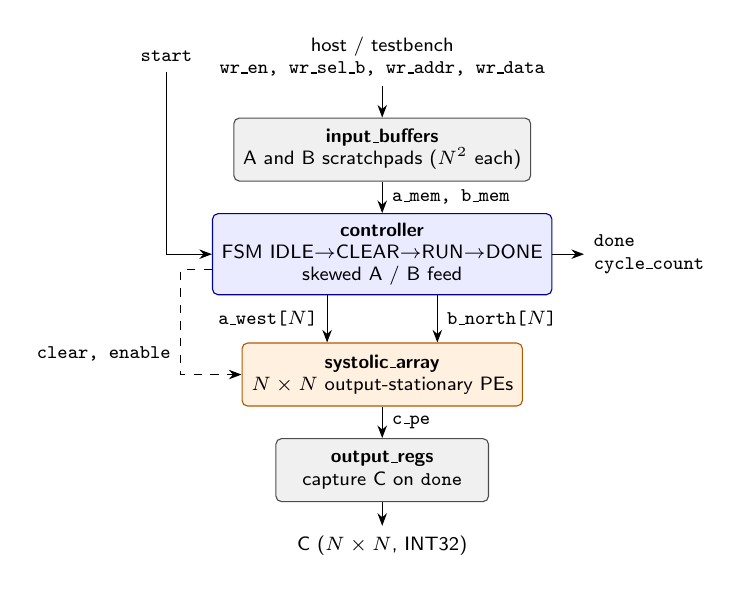
\begin{tikzpicture}[font=\sffamily\scriptsize, >={Stealth[length=1.6mm]},
  blk/.style={draw, rounded corners=2pt, align=center, minimum width=27mm, minimum height=8mm, fill=white},
  ctl/.style={blk, fill=blue!8, draw=blue!60!black},
  arr/.style={blk, fill=orange!12, draw=orange!70!black},
  mem/.style={blk, fill=gray!12, draw=gray!60!black}]
\node[align=center] (host) {host / testbench\\\texttt{wr\_en, wr\_sel\_b, wr\_addr, wr\_data}};
\node[mem, below=4mm of host] (buf) {\textbf{input\_buffers}\\A and B scratchpads ($N^2$ each)};
\node[ctl, below=4mm of buf] (ctl) {\textbf{controller}\\FSM IDLE$\to$CLEAR$\to$RUN$\to$DONE\\skewed A / B feed};
\node[arr, below=6mm of ctl] (sa) {\textbf{systolic\_array}\\$N\times N$ output-stationary PEs};
\node[mem, below=4mm of sa] (out) {\textbf{output\_regs}\\capture C on \texttt{done}};
\node[below=3mm of out, align=center] (c) {C ($N\times N$, INT32)};
\draw[->] (host) -- (buf);
\draw[->] (buf) -- node[right] {\texttt{a\_mem, b\_mem}} (ctl);
\draw[->] ([xshift=-7mm]ctl.south) -- node[left] {\texttt{a\_west[$N$]}} ([xshift=-7mm]sa.north);
\draw[->] ([xshift=7mm]ctl.south) -- node[right] {\texttt{b\_north[$N$]}} ([xshift=7mm]sa.north);
\draw[->] (sa) -- node[right] {\texttt{c\_pe}} (out);
\draw[->] (out) -- (c);
\node[left=1mm of host.west, anchor=east] (start) {\texttt{start}};
\draw[->] (start.south) |- (ctl.west);
\node[right=4mm of ctl.east, align=left] (dn) {\texttt{done}\\\texttt{cycle\_count}};
\draw[->] (ctl.east) -- (dn.west);
\draw[->, dashed] ([yshift=-2mm]ctl.west) -| ++(-4mm,-8mm) |- node[pos=0.25,left] {\texttt{clear, enable}} (sa.west);
\end{tikzpicture}
 & % (b) 4x4 output-stationary array with skewed inputs
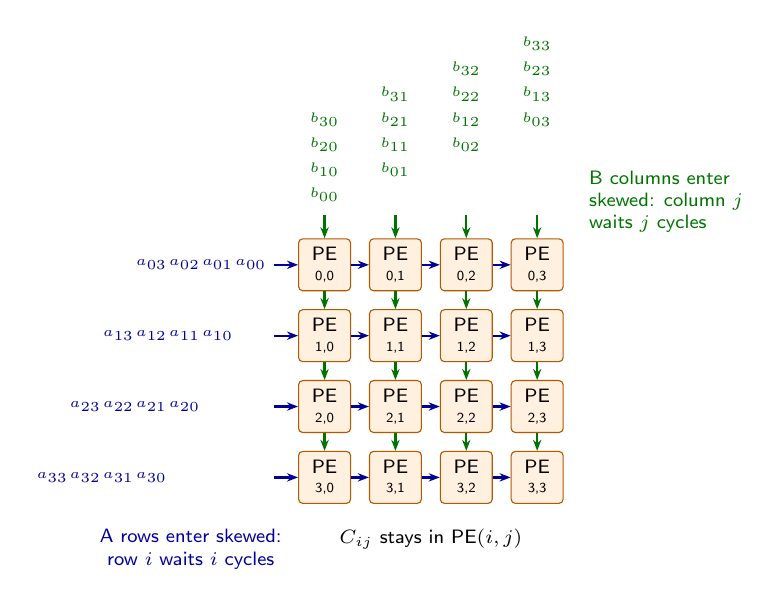
\begin{tikzpicture}[font=\sffamily\scriptsize, >={Stealth[length=1.4mm]}]
\def\s{9mm}
\foreach \i in {0,...,3} \foreach \j in {0,...,3} {
  \node[draw=orange!70!black, fill=orange!12, rounded corners=1.5pt, minimum size=6.6mm, inner sep=0, align=center]
    (p\i\j) at (\j*\s, -\i*\s) {PE\\[-1pt]\tiny\i,\j};
}
\foreach \i in {0,...,3} \foreach \j in {0,1,2} {
  \pgfmathtruncatemacro{\jn}{\j+1}
  \draw[->, thick, blue!60!black] (p\i\j.east) -- (p\i\jn.west);
}
\foreach \j in {0,...,3} \foreach \i in {0,1,2} {
  \pgfmathtruncatemacro{\in}{\i+1}
  \draw[->, thick, green!45!black] (p\i\j.south) -- (p\in\j.north);
}
% skewed A rows on the left: row i delayed by i slots
\foreach \i in {0,...,3} {
  \draw[->, thick, blue!60!black] ($(p\i0.west)+(-3mm,0)$) -- (p\i0.west);
  \foreach \k in {0,...,3} {
    \pgfmathsetlengthmacro{\x}{-6mm - (\k+\i)*4.2mm}
    \node[font=\sffamily\tiny, text=blue!60!black] at ($(p\i0.west)+(\x,0)$) {$a_{\i\k}$};
  }
}
% skewed B columns on top: column j delayed by j slots
\foreach \j in {0,...,3} {
  \draw[->, thick, green!45!black] ($(p0\j.north)+(0,3mm)$) -- (p0\j.north);
  \foreach \k in {0,...,3} {
    \pgfmathsetlengthmacro{\y}{5.5mm + (\k+\j)*3.2mm}
    \node[font=\sffamily\tiny, text=green!45!black] at ($(p0\j.north)+(0,\y)$) {$b_{\k\j}$};
  }
}
\node[font=\sffamily\scriptsize, align=center, text=blue!60!black, anchor=north] at ($(p30.south)+(-17mm,-2mm)$) {A rows enter skewed:\\row $i$ waits $i$ cycles};
\node[font=\sffamily\scriptsize, align=left, text=green!45!black, anchor=west] at ($(p03.east)+(2mm,8mm)$) {B columns enter\\skewed: column $j$\\waits $j$ cycles};
\node[font=\sffamily\scriptsize, align=center, anchor=north] at ($(p31.south)!0.5!(p32.south)+(0,-2mm)$) {$C_{ij}$ stays in PE$(i,j)$};
\end{tikzpicture}
\\[2pt]
\sffamily\small (a) Top-level hierarchy & \sffamily\small (b) $4\times4$ array and skewed dataflow
\end{tabular}}
\caption{Proposed accelerator. (a) Module hierarchy of \texttt{systolic\_top}. (b) Output-stationary dataflow: row $i$ of $A$ enters from the left delayed by $i$ cycles, column $j$ of $B$ enters from the top delayed by $j$ cycles, and $C_{ij}$ is accumulated inside PE$(i,j)$.}
\label{fig:arch}
\end{figure*}

\subsection{Choice of Dataflow}
We chose output-stationary dataflow because it is the easiest to reason about: PE$(i,j)$ owns exactly one output $C_{ij}$, and no partial sums ever leave the array until the end. The known cost is lower PE utilisation for a single matrix, because PEs are idle while the data wave fills and drains the array (quantified in Section~\ref{sec:metrics}).

\subsection{MAC Unit and Processing Element}

\begin{figure}[t]
\centering
\resizebox{0.92\columnwidth}{!}{% (c) Output-stationary processing element
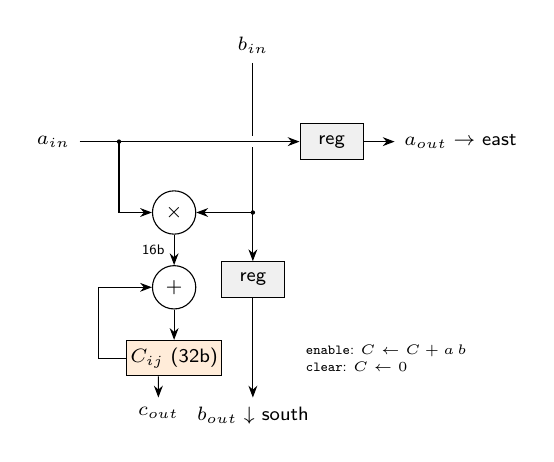
\begin{tikzpicture}[font=\sffamily\scriptsize, >={Stealth[length=1.5mm]},
  r/.style={draw, fill=gray!12, minimum width=8mm, minimum height=4.5mm, inner sep=1pt},
  op/.style={draw, circle, minimum size=5.5mm, inner sep=0, fill=white}]
\node[anchor=east] (ain) at (0,0) {$a_{in}$};
\node[r] (ra) at (3.2,0) {reg};
\node[anchor=west] (aout) at (4.0,0) {$a_{out}\to$ east};
\node[anchor=south] (bin) at (2.2,1.0) {$b_{in}$};
\node[op] (mul) at (1.2,-0.9) {$\times$};
\node[op] (add) at (1.2,-1.85) {$+$};
\node[r, fill=orange!15, minimum width=12mm] (acc) at (1.2,-2.75) {$C_{ij}$ (32b)};
\node[r] (rb) at (2.2,-1.75) {reg};
\node[anchor=north] (bout) at (2.2,-3.25) {$b_{out}\downarrow$ south};
\node[anchor=north] (cout) at (1.0,-3.25) {$c_{out}$};
% a path
\draw[->] (ain.east) -- (ra.west);
\draw[->] (ra.east) -- (aout.west);
\fill (0.5,0) circle (0.8pt);
\draw[->] (0.5,0) |- (mul.west);
% b path (crosses the a line)
\draw (bin.south) -- (2.2,0.07);
\draw (2.2,-0.07) -- (2.2,-0.9);
\fill (2.2,-0.9) circle (0.8pt);
\draw[->] (2.2,-0.9) -- (mul.east);
\draw[->] (2.2,-0.9) -- (rb.north);
\draw[->] (rb.south) -- (bout.north);
% MAC
\draw[->] (mul) -- node[left, font=\sffamily\tiny] {16b} (add);
\draw[->] (add) -- (acc);
\draw[->] (acc.west) -- ++(-0.35,0) |- (add.west);
\draw[->] ([xshift=-2mm]acc.south) -- (cout.north);
\node[anchor=west, align=left, font=\sffamily\tiny] at (2.75,-2.75) {\texttt{enable}: $C \leftarrow C + a\,b$\\\texttt{clear}: $C \leftarrow 0$};
\end{tikzpicture}
}
\caption{One processing element: a signed $8\times8$-bit multiplier, a 32-bit accumulator holding $C_{ij}$, and two pipeline registers that forward $a$ east and $b$ south.}
\label{fig:pe}
\end{figure}

The \texttt{mac\_unit} computes, combinationally,
\begin{equation}
y = acc + \operatorname{sext}_{32}(a \times b),
\end{equation}
where $a, b$ are signed 8-bit values, the full 16-bit signed product is sign-extended to 32 bits, and $acc$ is the current sum. The \texttt{pe} (Fig.~\ref{fig:pe}) adds three registers: on every clock edge it forwards $a_{out} \leftarrow a_{in}$ and $b_{out} \leftarrow b_{in}$; if \texttt{clear} is high it sets $C \leftarrow 0$, otherwise if \texttt{enable} is high it updates $C \leftarrow y$.

\emph{Overflow.} The largest product magnitude is $(-128)\times(-128) = 16{,}384$, so after $N$ accumulations $|C| \le 16{,}384\,N$. A signed 32-bit accumulator therefore cannot overflow for any $N \le 131{,}071$, far beyond the sizes used here.

\subsection{Systolic Array}
The \texttt{systolic\_array} module uses Verilog \texttt{generate} loops to build an $N\times N$ mesh of PEs. The $a_{out}$ of PE$(i,j)$ connects to the $a_{in}$ of PE$(i,j{+}1)$, and the $b_{out}$ of PE$(i,j)$ connects to the $b_{in}$ of PE$(i{+}1,j)$. All PEs share \texttt{clear} and \texttt{enable}.

\subsection{Controller and Skew Schedule}
The controller is a four-state finite-state machine: \texttt{IDLE} $\rightarrow$ \texttt{CLEAR} $\rightarrow$ \texttt{RUN} $\rightarrow$ \texttt{DONE}. Let $t$ be the injection step at the array boundary. The controller places
\begin{equation}
\begin{aligned}
A_{ik} &\text{ on } \texttt{a\_west}[i] \text{ at step } t = i + k,\\
B_{kj} &\text{ on } \texttt{b\_north}[j] \text{ at step } t = j + k.
\end{aligned}
\end{equation}
Because each PE adds one cycle of delay in each direction, $A_{ik}$ reaches column $j$ after $j$ more cycles and $B_{kj}$ reaches row $i$ after $i$ more cycles. Both therefore arrive at PE$(i,j)$ at the same step
\begin{equation}
r = i + j + k,
\end{equation}
which is exactly the pair that PE$(i,j)$ needs for the term $A_{ik}B_{kj}$ of $C_{ij}$. The last pair meets at PE$(N{-}1,N{-}1)$ for $k = N{-}1$, at $r = 3N - 3$. Counting one \texttt{CLEAR} cycle, $3N-2$ \texttt{RUN} cycles and the cycle that raises \texttt{done}, the latency from \texttt{start} to \texttt{done} is
\begin{equation}
L_{\text{sys}} = 3N \text{ cycles} \quad (12 \text{ for } N = 4).
\end{equation}
Outside its valid window each boundary input is driven with zero, so extra cycles add nothing to the sums. A 16-bit \texttt{cycle\_count} output reports the measured latency.

\subsection{Buffers and Output Registers}
\texttt{input\_buffers} holds $A$ and $B$ in row-major order ($N^2$ entries each) and is written one element per cycle through \texttt{wr\_en}, \texttt{wr\_sel\_b} (0 = $A$, 1 = $B$), \texttt{wr\_addr} and \texttt{wr\_data}. \texttt{output\_regs} copies all $N^2$ accumulators when \texttt{done} is high, so the result stays stable while the array is reused.

\subsection{Sequential Baseline}
For a fair comparison, \texttt{seq\_matmul} uses the same buffers and widths but only one multiplier. It loops over $i$, $j$ and $k$ and performs one MAC per cycle, so after one clear cycle its latency is
\begin{equation}
L_{\text{seq}} = N^3 + 1 \text{ cycles} \quad (65 \text{ for } N = 4).
\end{equation}

\subsection{Performance Metrics}
\label{sec:metrics}
For one $N\times N$ multiplication ($N^3$ MACs):
\begin{align}
\text{Speed-up} &= \frac{L_{\text{seq}}}{L_{\text{sys}}} = \frac{N^3 + 1}{3N} \approx \frac{N^2}{3},\\
\text{Throughput} &= \frac{N^3}{L_{\text{sys}}} = \frac{N^2}{3}\ \text{MACs/cycle},\\
\text{PE utilisation} &= \frac{N^3}{N^2 \cdot L_{\text{sys}}} = \frac{1}{3} \approx 33\%.
\end{align}
The one-third utilisation is the fill-and-drain cost of output-stationary dataflow for a single matrix: each PE is busy for only $N$ of the $3N$ cycles. The speed-up grows roughly with $N^2$, at the cost of $N^2$ multipliers instead of one.

\subsection{Verification Plan}
All testbenches are self-checking and print PASS or FAIL:
\begin{itemize}
\item \texttt{tb\_pe}: 21 directed checks on one PE, including $3\times4 = 12$, $-2\times5 = -10$, the extremes $127\times127 = 16{,}129$, $(-128)\times(-128) = 16{,}384$ and $(-128)\times127 = -16{,}256$, signed accumulation over two and four steps (a full dot product for $N = 4$), clear, priority of \texttt{clear} over \texttt{enable}, hold when \texttt{enable} is low, and pass-through of $a$ and $b$.
\item \texttt{tb\_systolic}: for $N = 4$ and $N = 3$, an identity case, a zero case, a corner case with the extreme values 127 and $-128$, and 20 random signed matrices; every output element is compared with a software golden model, and the latency is checked to be exactly $3N$ (46 tests in total).
\item \texttt{tb\_compare}: the systolic array and the sequential baseline run on the same matrices; their results must match and their cycle counts must be 12 and 65.
\item \texttt{tb\_demo}: a readable signed $4\times4$ example that prints $A$, $B$, the hardware result and the expected result, used in the demonstration video.
\end{itemize}

\subsection{Tool Flow}
Verilog RTL is simulated with Icarus Verilog~\cite{iverilog} (\texttt{make test}), waveforms are inspected in GTKWave with a saved signal layout (\texttt{waveforms/tb\_demo.gtkw}; Fig.~\ref{fig:wave} is drawn from the same VCD file by \texttt{scripts/plot\_waveform.py}), and synthesis for a Xilinx 7-series FPGA is done in Vivado on the lab machines. For an early resource estimate we also synthesised a single PE with the open-source Yosys tool~\cite{yosys}.

% =====================================================================
\section{Prototype Status and Preliminary Results}

The register-transfer-level (RTL) design and its verification are complete. Table~\ref{tab:status} lists what is done and what remains for Phase II.

\begin{table}[t]
\caption{Implementation status at the end of Phase I}
\label{tab:status}
\centering
\scriptsize
\renewcommand{\arraystretch}{1.12}
\begin{tabularx}{\columnwidth}{@{}Yl@{}}
\toprule
\textbf{Item} & \textbf{Status} \\
\midrule
Eight synthesizable RTL modules (\texttt{rtl/}) & Done \\
PE testbench: 21/21 checks pass & Done \\
System testbench: 46/46 tests pass ($N = 3$ and 4) & Done \\
Systolic vs.\ sequential comparison: results match & Done \\
Demo testbench, GTKWave save file and waveform analysis & Done \\
Yosys estimate for one PE (Xilinx 7-series) & Done \\
Vivado synthesis of the full design: LUT, FF, DSP, $F_{max}$ & Phase II \\
Larger $N$, back-to-back matrices, optional board demo & Phase II \\
\bottomrule
\end{tabularx}
\end{table}

\subsection{Latency and Speed-up}
Table~\ref{tab:results} shows the cycle counts measured in simulation. They match the formulas of Section~\ref{sec:metrics} exactly.

\begin{table}[t]
\caption{Measured latency (Icarus Verilog simulation)}
\label{tab:results}
\centering
\scriptsize
\renewcommand{\arraystretch}{1.15}
\begin{tabular}{@{}lccccc@{}}
\toprule
$N$ & \textbf{Systolic} & \textbf{Sequential} & \textbf{Speed-up} & \textbf{MACs/cycle} & \textbf{PE util.} \\
 & (cycles) & (cycles) & & (sys.\ / seq.) & \\
\midrule
3 & 9 & 28 & $3.11\times$ & 3.00 / 0.96 & 33\% \\
4 & 12 & 65 & $5.42\times$ & 5.33 / 0.98 & 33\% \\
\bottomrule
\end{tabular}
\end{table}

\subsection{Functional Correctness}
All 21 PE checks, all 46 system tests and the comparison test pass, so the array produces bit-exact results against the golden model for identity, zero, extreme-value and random signed inputs. In the demo example, with $A$ holding 1 to 16 and $B$ holding small signed values, the hardware output equals the software reference element by element (for instance $C_{00} = 6$ and $C_{33} = 31$).

\subsection{Data Propagation in the Waveform}
Fig.~\ref{fig:wave} shows the simulated waveform of the demo. After \texttt{start}, the FSM spends one cycle in \texttt{CLEAR} and then enters \texttt{RUN}. Row 0 of $A$ (1, 2, 3, 4) enters \texttt{a\_west[0]} first, and each following row starts one cycle later; the columns of $B$ are skewed the same way on \texttt{b\_north}. PE$(0,0)$ finishes its sum ($1 + 0 + 9 - 4 = 6$) early, while the corner PE$(3,3)$ receives its first pair last and reaches 31 at the end. \texttt{done} rises at cycle 12, exactly $3N$.

\begin{figure*}[t]
\centering
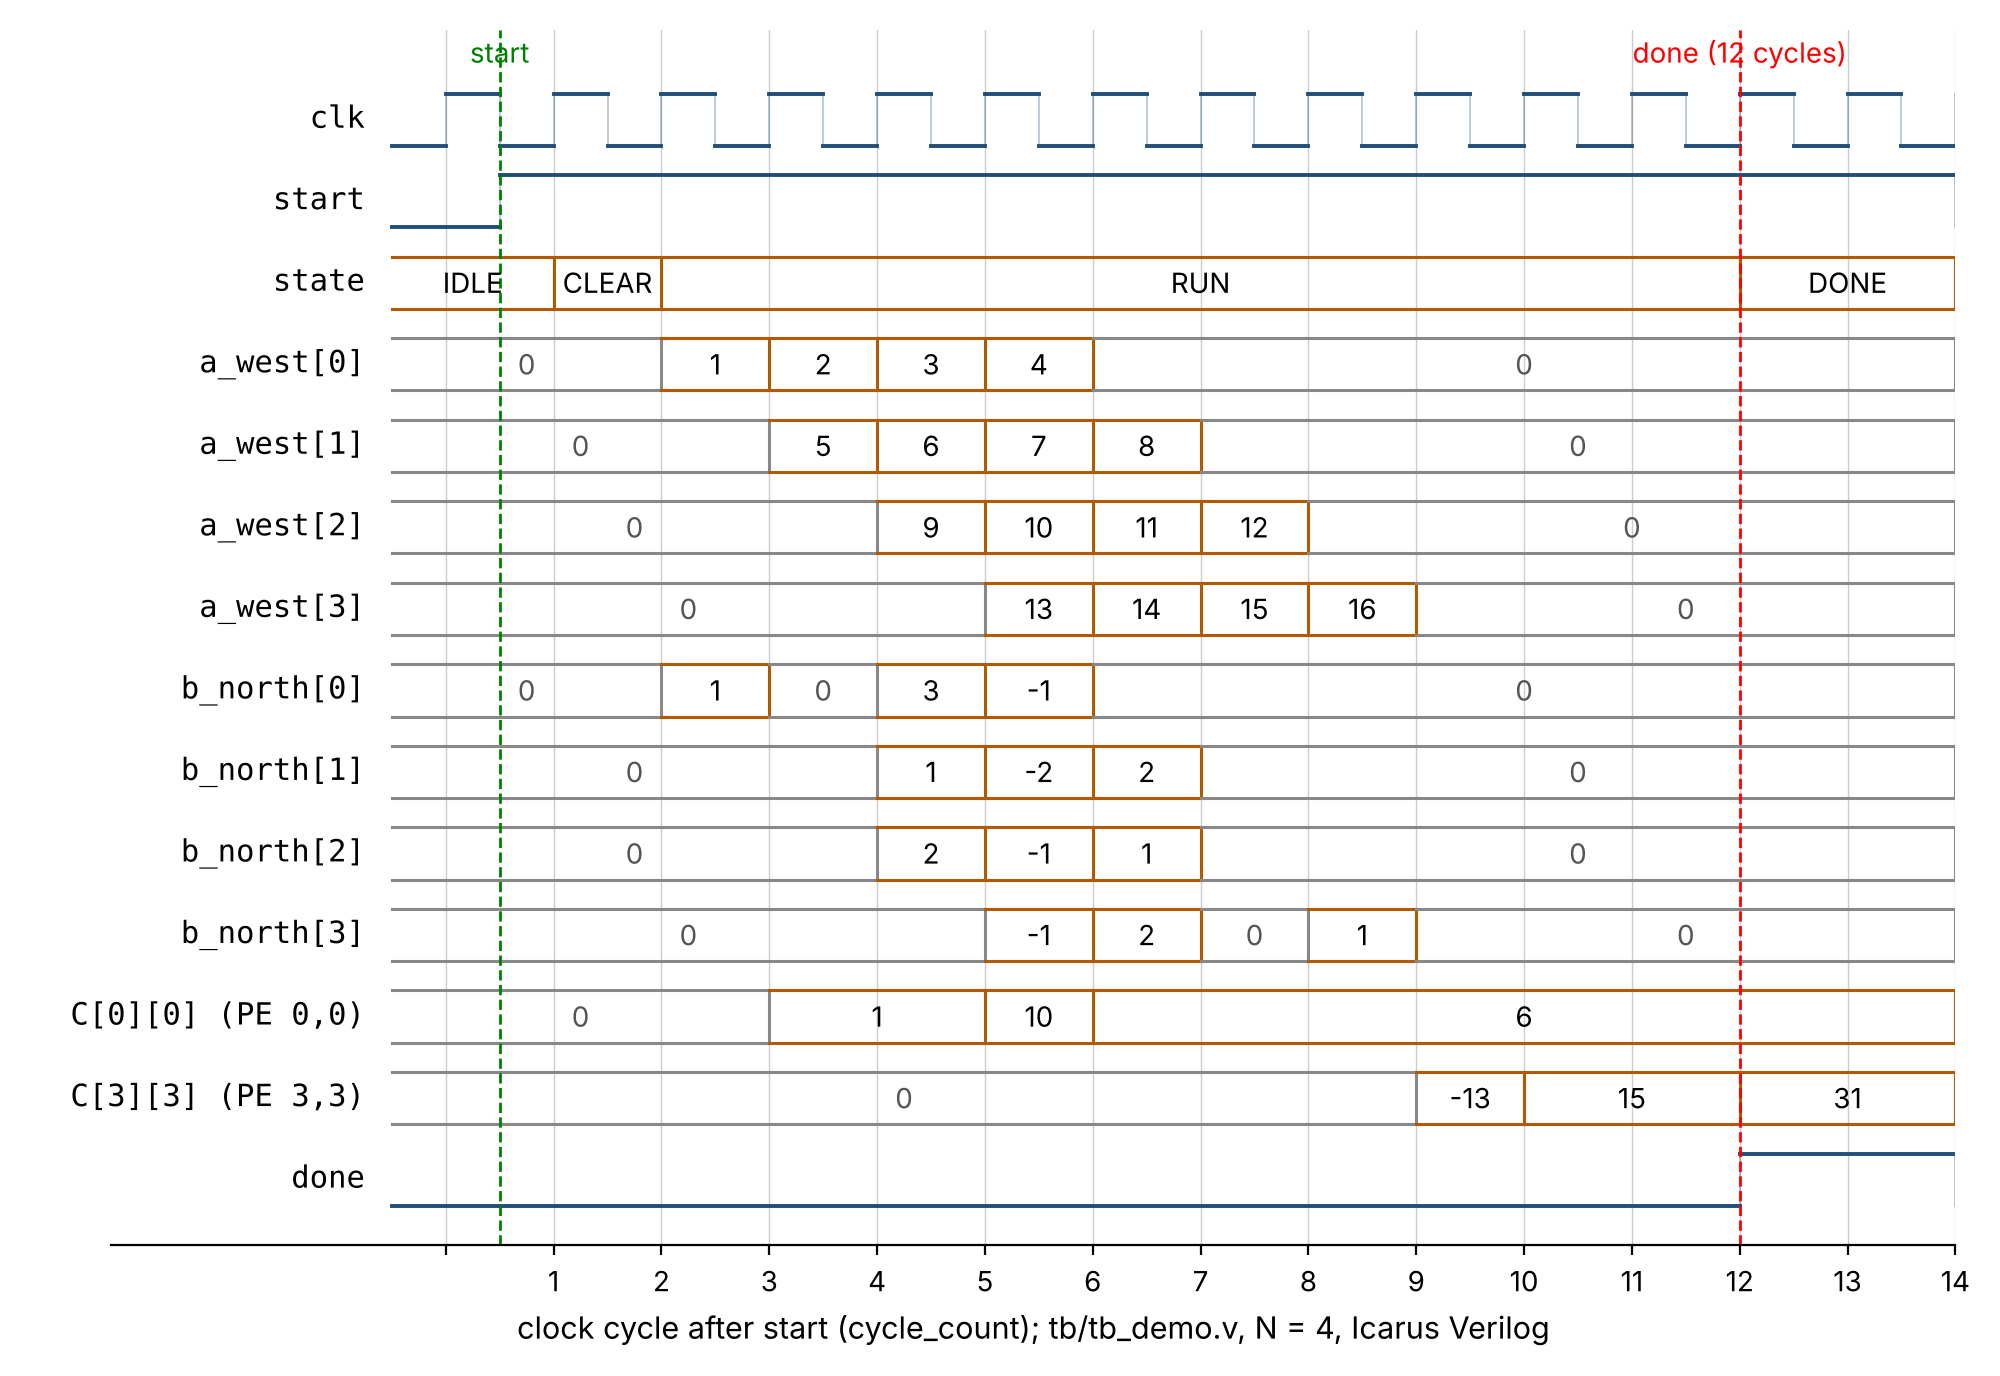
\includegraphics[width=0.9\textwidth]{waveform.png}
\caption{Simulated waveform of \texttt{tb\_demo} ($N = 4$), drawn from the VCD file. The staircase pattern of \texttt{a\_west} and \texttt{b\_north} is the skew that makes matching operands meet inside each PE; zero values are shown in grey.}
\label{fig:wave}
\end{figure*}

\subsection{Early Resource Estimate}
Yosys synthesis of one PE for a Xilinx 7-series device maps the multiplier and adder to one DSP48E1 slice and uses 48 flip-flops ($8 + 8$ pipeline bits and the 32-bit accumulator) and 32 LUTs. A $4\times4$ array therefore needs about 16 DSP slices and 768 flip-flops for the PEs alone, before the controller and buffers, compared with one multiplier for the sequential baseline. This is an estimate only; the full-design numbers and the maximum clock frequency will come from Vivado in Phase II.

% =====================================================================
\section{Plan for Phase II}
\begin{enumerate}
\item \textbf{FPGA synthesis and timing:} run Vivado on the full \texttt{systolic\_top} ($N = 4$), report LUTs, flip-flops, DSP slices and $F_{max}$, and compare with the sequential baseline (area versus speed).
\item \textbf{Scaling study:} extend the testbenches to more array sizes (for example $N = 2$ to 8) and confirm that latency stays $3N$ and speed-up grows as $N^2/3$.
\item \textbf{Higher utilisation:} overlap the drain of one matrix with the fill of the next so that back-to-back multiplications keep more PEs busy; compare with weight-stationary behaviour.
\item \textbf{Optional:} tiling for matrices larger than the array, and a board demonstration with on-chip logic analyser (ILA) captures.
\item \textbf{Final IEEE report} with Results and Discussion and Conclusion, and preparation for the project interview by all members.
\end{enumerate}

% =====================================================================
\section{Individual Contributions}

\begin{table}[h]
\caption{Individual contributions}
\label{tab:contrib}
\centering
\scriptsize
\renewcommand{\arraystretch}{1.2}
\begin{tabularx}{\columnwidth}{@{}L{1.55cm}Y@{}}
\toprule
\textbf{Member} & \textbf{Contribution} \\
\midrule
Shivam Mittal (team lead) & Architecture and dataflow choice; controller FSM and skew schedule; top-level integration (\texttt{systolic\_top}); repository and Makefile build flow. \\
Divya Singh & MAC unit and output-stationary PE (signed arithmetic, sign extension, clear/enable logic); PE directed testbench. \\
Sanath Waraikar & $N\times N$ array mesh with \texttt{generate} loops; input buffers and output registers. \\
Aryan & System verification: golden-model testbench (identity, zero, corner, random), systolic-versus-sequential comparison, waveform analysis. \\
Khushi Batra & Literature review; sequential baseline module; performance metrics (latency, throughput, utilisation); documentation. \\
\bottomrule
\end{tabularx}
\end{table}

% =====================================================================
\begin{thebibliography}{99}
\footnotesize

\bibitem{kung1979}
H.~T. Kung and C.~E. Leiserson, ``Systolic arrays (for VLSI),'' in \emph{Sparse Matrix Proceedings 1978}, I.~S. Duff and G.~W. Stewart, Eds. Philadelphia, PA, USA: SIAM, 1979, pp.~256--282.

\bibitem{kung1982}
H.~T. Kung, ``Why systolic architectures?'' \emph{Computer}, vol.~15, no.~1, pp.~37--46, Jan. 1982, doi: 10.1109/MC.1982.1653825.

\bibitem{jouppi2017}
N.~P. Jouppi \emph{et al.}, ``In-datacenter performance analysis of a tensor processing unit,'' in \emph{Proc. 44th Annu. Int. Symp. Computer Architecture (ISCA)}, 2017, pp.~1--12. [Online]. Available: \url{https://arxiv.org/abs/1704.04760}

\bibitem{chen2016}
Y.-H. Chen, J.~Emer, and V.~Sze, ``Eyeriss: A spatial architecture for energy-efficient dataflow for convolutional neural networks,'' in \emph{Proc. 43rd Annu. Int. Symp. Computer Architecture (ISCA)}, 2016, pp.~367--379.

\bibitem{sze2017}
V.~Sze, Y.-H. Chen, T.-J. Yang, and J.~S. Emer, ``Efficient processing of deep neural networks: A tutorial and survey,'' \emph{Proc. IEEE}, vol.~105, no.~12, pp.~2295--2329, Dec. 2017. [Online]. Available: \url{https://arxiv.org/abs/1703.09039}

\bibitem{genc2021}
H.~Genc \emph{et al.}, ``Gemmini: Enabling systematic deep-learning architecture evaluation via full-stack integration,'' in \emph{Proc. 58th ACM/IEEE Design Automation Conf. (DAC)}, 2021. [Online]. Available: \url{https://github.com/ucb-bar/gemmini}

\bibitem{samajdar2018}
A.~Samajdar, Y.~Zhu, P.~Whatmough, M.~Mattina, and T.~Krishna, ``SCALE-Sim: Systolic CNN accelerator simulator,'' \emph{arXiv preprint arXiv:1811.02883}, 2018. [Online]. Available: \url{https://github.com/ARM-software/SCALE-Sim}

\bibitem{xilinx_ug479}
Xilinx Inc., ``7 Series DSP48E1 Slice User Guide,'' UG479. [Online]. Available: \url{https://docs.amd.com/v/u/en-US/ug479_7Series_DSP48E1}

\bibitem{iverilog}
S.~Williams, ``Icarus Verilog.'' [Online]. Available: \url{https://steveicarus.github.io/iverilog/}

\bibitem{yosys}
C.~Wolf, ``Yosys Open SYnthesis Suite.'' [Online]. Available: \url{https://yosyshq.net/yosys/}

\end{thebibliography}

\end{document}
